%% Overleaf			
%% Software Manual and Technical Document Template	
%% 									
%% This provides an example of a software manual created in Overleaf.

\documentclass{ol-softwaremanual}

% Packages used in this example
\usepackage{graphicx}  % for including images
\usepackage{microtype} % for typographical enhancements
\usepackage{minted}    % for code listings
\usepackage{amsmath}   % for equations and mathematics
\setminted{style=friendly,fontsize=\small}
\renewcommand{\listoflistingscaption}{List of Code Listings}
\usepackage{hyperref}  % for hyperlinks
\usepackage[a4paper,top=4.2cm,bottom=4.2cm,left=3.5cm,right=3.5cm]{geometry} % for setting page size and margins

% Custom macros used in this example document
\newcommand{\doclink}[2]{\href{#1}{#2}\footnote{\url{#1}}}
\newcommand{\cs}[1]{\texttt{\textbackslash #1}}

% Frontmatter data; appears on title page
\title{Web Data Extraction System Design}
\version{1.0.0}
\author{Trinh Xuan Tam}
\softwarelogo{
\includegraphics[width=8cm]{logo}}

\begin{document}

\maketitle

\tableofcontents
% \listoflistings
\newpage

\section{Assignment}

Design (technical document) a system that processes an infinite
stream of data:
\begin{itemize}
  \item Each record comes as a tuple(url, html content)
  \item Extract and store the occurrences of: urls, hosts, top-level-domains, in/out links of the page
\end{itemize}

We have one machine that has enough disk space but limited memory. Write a design document to describe the system architecture and data structures as building blocks.

\section{System Design}
This section outlines the overall architecture and specific design choices for the system. It provides a comprehensive view of how the various components of the system interact and how data flows through the system.

\subsection{System Architecture Overview}

\begin{figure}[h]
\centering
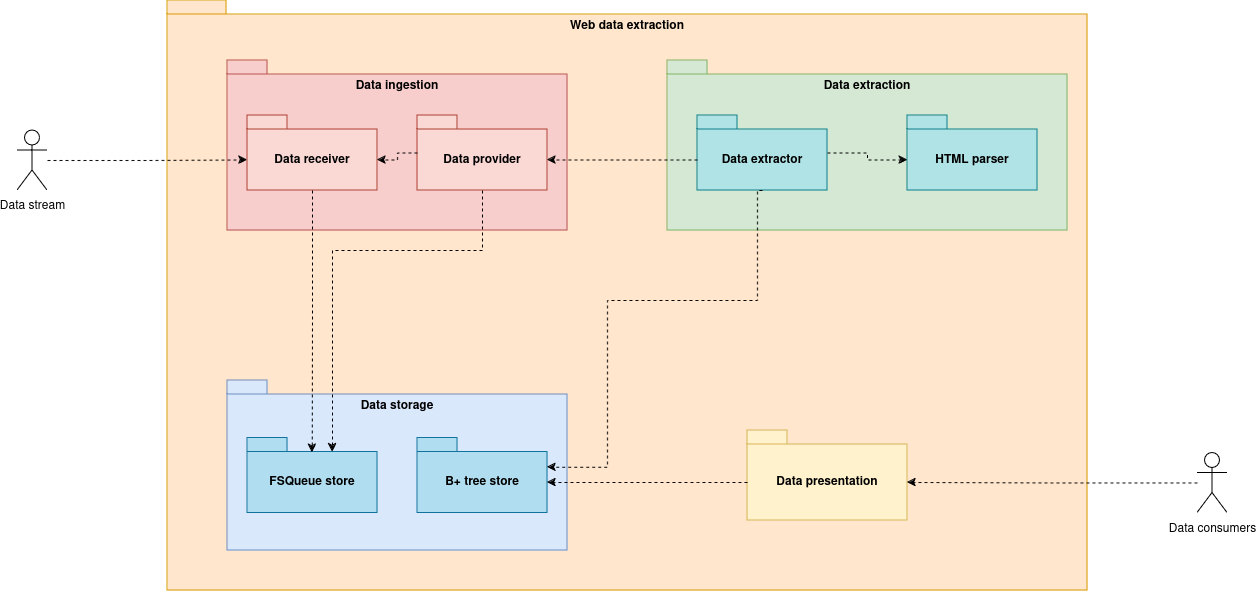
\includegraphics[width=\textwidth]{images/package.png}
\caption{\label{fig:package-diagram} Package diagram of the proposed system.}
\end{figure}

The package diagram presented above outlines the main components of the proposed system along with their dependencies. It is assumed that the underlying infrastructure, including data streaming and consumption, is already in place. The diagram specifically emphasizes the design of a service dedicated to extracting data from the stream.

\subsection{Data storage module}

This module is primarily responsible for managing all interactions with the data storage systems, which might include both file-based and database storage mechanisms. It employs various algorithms and data structures optimized for performance and reliability, focusing on the complexities of handling large-scale data efficiently.

\subsubsection{File system based queue}

This module implements a queue that is based on a file. It allows the system to push data and pop data from the file. Additionally, it requires the caller to define a serialization mechanism to JSON. The implementation could use JSON encoding and read a file line by line, which provides a simple yet effective way to handle data without needing a complex database system.

The file system-based queue uses a simple text file to store JSON serialized objects. Each line in the file represents a queue item. The queue then store each json line by line in chunks of predefined size. The queue maintains a reference to the head and tail chunks.

\paragraph{Implementation Details}
\begin{enumerate}
    \item \textbf{Initialization}: On initialization, the queue checks for the existence of the queue file. If not found, it creates an empty file to begin operations.
    \item \textbf{Push Operation}: To add an item to the queue, the item is serialized into a JSON string and appended to the end of the file followed by a newline. This ensures that each entry remains on a separate line for easy retrieval.
    \item \textbf{Pop Operation}: To remove an item from the queue, read the last line of the file. This line is then removed and the file is rewritten without this line. The data from the popped line is deserialized and returned to the caller.
    \item \textbf{End-of-Life}: When the queue is no longer needed, a cleanup operation can be performed to delete the queue file, ensuring that no residual data is left on the system.
\end{enumerate}

\pagebreak

\subsubsection{B+ tree}

The B+ tree component is designed to efficiently index and store JSON objects based on keys converted to integer representations. The keys are distributed across a range, with each range associated with a specific file chunk that stores multiple JSON objects.

\paragraph{Implementation Details}
\begin{itemize}
    \item \textbf{Key Conversion}: Each key, regardless of its original format, is converted to an integer representation using a given hash function. This integer determines which node (and consequently which file chunk) the corresponding JSON object should be stored in.
    \item \textbf{Node Structure}: Nodes are divided into leaf and internal types. Internal nodes store keys and pointers to child nodes, while leaf nodes store ranges of keys and pointers to file chunks.
    \item \textbf{File Structure}: Each leaf node points to a file chunk where JSON objects are stored line by line. Each file chunk corresponds to a specific range of keys.
    \item \textbf{Operations}:
    \begin{itemize}
        \item \textbf{Insertion}: Inserts new keys by locating the correct leaf node based on the key's integer value, and appending the JSON object to the appropriate file chunk.
        \item \textbf{Deletion}: Removes keys by locating and editing the appropriate file chunk, removing the specific JSON object line.
        \item \textbf{Search}: Finds keys by hashing to an integer and directly accessing the file chunk to search through the stored JSON lines. Additionally, caching of the file chunk can be implemented to reduce the amount of IO operations.
    \end{itemize}
    \item \textbf{Persistence and Recovery}: Node changes are written back to disk immediately to ensure data integrity, with recovery mechanisms in place to rebuild the tree from disk in case of system restarts.
\end{itemize}


\subsection{Data ingestion module}
The Data Ingestion Module is crucial for managing the intake and initial handling of the infinite data stream, which consists of tuples containing URLs and their corresponding HTML content. This module ensures that data is accepted smoothly, buffered efficiently, and then made available to other parts of the system as needed, while being memory efficient.

\subsubsection{Data Receiver}
The Data Receiver is responsible for continuously accepting data from the incoming stream and temporarily storing it in a buffer. This component is designed to handle high-volume data streams efficiently.

\paragraph{Implementation Details}
\begin{itemize}
    \item \textbf{Buffering}: The receiver includes a buffer that temporarily stores incoming (URL, HTML) tuples. The buffer size is predefined based on system performance evaluations and the typical data rate.
    \item \textbf{Bulk Insertion}: Once the buffer's content size exceeds a certain quota, the Data Receiver performs a bulk insertion of its contents into the previously described File-based Queue. This method ensures that the system can handle high volumes of stream data even with limited memory.
\end{itemize}

\subsubsection{Data Provider}
The Data Provider acts as an intermediary between the data storage components and other modules that require data for processing.

\paragraph{Implementation Details}
\begin{itemize}
    \item \textbf{Queue Monitoring}: Continuously checks the File-based Queue to determine if data is available. If the queue is not empty, it retrieves data by popping items from the queue.
    \item \textbf{Direct Access}: In situations where the File-based Queue is empty, the Data Provider accesses data directly from the Data Receiver's buffer. This ensures that data processing modules can operate without interruption, even when the queue mechanisms are temporarily depleted.
\end{itemize}

\subsection{Data extraction module}
The Data Extraction Module is responsible for processing HTML content to extract valuable data such as URLs, hosts, top-level domains, and in/out links. This module has two main submodules that specialize in different aspects of the data extraction process.

\subsubsection{HTML Parser}
The HTML Parser submodule provides a simplified interface for extracting specific HTML elements from web pages. Its primary goal is to enable efficient and accurate data parsing from complex HTML structures.

\paragraph{Implementation Details}
\begin{itemize}
    \item \textbf{Parsing Engine}: Utilizes a robust HTML parsing library, such as Beautiful Soup or lxml, which offers extensive capabilities for navigating, searching, and modifying the parse tree.
    \item \textbf{Element Retrieval}: Implements methods to specifically retrieve anchor tags, headers, and other relevant HTML elements that contain the targeted data such as URLs and metadata.
\end{itemize}

\subsubsection{Data Extractor}
The Data Extractor submodule takes input from the Data Provider Module, utilizes the HTML Parser to extract the necessary data, and subsequently forms a JSON object with all occurrences, which is then stored in the B+ tree.

\paragraph{Implementation Details}
\begin{itemize}
    \item \textbf{Data Flow}: Receives (URL, HTML) tuples from the Data Provider, which are then fed into the HTML Parser for data extraction.
    \item \textbf{Extraction Process}: Extracts URLs, hosts, TLDs, and in/out links based on the HTML content parsed. Each URL and its components are analyzed to categorize them as either inbound or outbound links.
    \item \textbf{JSON Formation}: After extraction, all occurrences are compiled into a structured JSON object. The structured JSON objects are then stored in the B+ tree where the key will be the given url from the tuple.
\end{itemize}

\subsection{Data presentation module}
The Data Presentation Module is designed to provide accessible and interpretable views of the data stored within the B+ tree. This module serves as the interface between the stored data and end users or other applications, facilitating easy access to structured information.

\subsubsection{Overview}
The primary function of this module is to read data from the B+ tree and present it in various formats that are useful for analysis, reporting, or further processing. It acts as the visualization layer of the system, where data is not only retrieved but also formatted for consumption.

\paragraph{Implementation Details}
\begin{itemize}
    \item \textbf{Data Retrieval}: Implements functions to query the B+ tree, extracting data based on specific keys or ranges of keys. This capability is crucial for supporting complex queries that end users might require.
    \item \textbf{View Generation}: Based on the retrieved data, this submodule can generate different views, such as lists, tables, or even graphical representations. These views are dynamically created based on user queries or predefined display settings.
\end{itemize}

\subsection{Summary}
This system is designed to process and manage an infinite stream of web data efficiently, even on a machine with limited memory. Each module within the system plays a critical role in ensuring that data is handled efficiently from ingestion to presentation.

\subsubsection{Efficient Data Handling}
\begin{itemize}
    \item The \textbf{Data Ingestion Module} uses buffering and bulk insertion strategies to manage high volumes of incoming data without overloading the system's memory. This allows the system to handle bursts of data efficiently.
    \item The \textbf{Data Storage Module}, including both the file-based queue and the B+ tree, optimizes data storage and access patterns. The file-based queue minimizes overhead by storing data linearly and using a simple JSON serialization for persistence, while the B+ tree provides efficient indexing and retrieval capabilities for large datasets.
\end{itemize}

\subsubsection{Memory Optimization}
\begin{itemize}
    \item \textbf{Data structures and algorithms} used in the system are selected based on their low memory requirements and high efficiency. For instance, the B+ tree minimizes disk I/O by organizing data into blocks and storing indices in memory, which accelerates search operations without consuming excessive memory.
    \item The use of a file-based queue reduces the need for complex database management systems that typically require more memory and computational resources. This approach leverages the filesystem for data persistence, which is generally more memory-efficient and simpler to scale on a single machine.
\end{itemize}

\end{document}
